\documentclass[twoside,twocolumn]{article}

\usepackage{blindtext} 
\usepackage{graphicx}
\usepackage[sc]{mathpazo} 
\usepackage[T1]{fontenc} 
\linespread{1.05} 
\usepackage{microtype} 
\usepackage[utf8]{inputenc} 
\usepackage[spanish,english]{babel} 
\usepackage[hmarginratio=1:1,top=32mm,columnsep=20pt]{geometry} 
\usepackage[hang, small,labelfont=bf,up,textfont=it,up]{caption} 
\usepackage{booktabs} 
\usepackage{lettrine} 
\usepackage{enumitem} 

\usepackage{titling}
\usepackage{hyperref} 
\usepackage{listings}
\usepackage[table,xcdraw]{xcolor}

\lstdefinestyle{sharpc}{language=[Sharp]C, frame=lr, rulecolor=\color{blue!80!black}}

\setlist[itemize]{noitemsep} 

\usepackage{abstract} 
\renewcommand{\abstractnamefont}{\normalfont\bfseries} 
\renewcommand{\abstracttextfont}{\normalfont\small\itshape} 

\usepackage{titlesec} 
\renewcommand\thesection{\Roman{section}} % 
\renewcommand\thesubsection{\roman{subsection}} 
\titleformat{\section}[block]{\large\scshape\centering}{\thesection.}{1em}{} 
\titleformat{\subsection}[block]{\large}{\thesubsection.}{1em}{} 

\usepackage{fancyhdr} 
\pagestyle{fancy} 
\fancyhead{} 
\fancyfoot{} 
\fancyhead[C]{Herramientas de gestión de pruebas $\bullet$ Enero 2021 $\bullet$ } 
\fancyfoot[RO,LE]{\thepage} 

%----------------------------------------------------------------------------------------
%	TILULOS
%----------------------------------------------------------------------------------------


\setlength{\droptitle}{-4\baselineskip} 

\pretitle{\begin{center}\Huge\bfseries} 
\posttitle{\end{center}} 
\title{Herramientas de gestión de pruebas} 
\author{Percy Taquila Carazas, Katerin Merino Quispe, Abraham Lipa Calabilla,
\\Edwart Balcon Coahila, Lisbeth Espinoza Caso}
\date{\today} 
\renewcommand{\maketitlehookd}{

\selectlanguage{english}
\begin{abstract}
\noindent 
The Test Management Tool is the tool that provides support for the test management and control of part of the testing process. Often it has multiple capabilities, such as managing test support products, test planning, results recording, process tracking, incident management, and test reporting.
They have different approaches to testing and therefore have different sets of features. They are typically used to maintain and schedule manual tests, run or collect automated test execution data, manage multiple environments, and enter information on found defects.
\end{abstract}


\selectlanguage{spanish}
\begin{abstract}
\noindent 
Las Herramienta de gestión de pruebas es la herramienta que proporciona soporte a la gestión de pruebas y control de parte del proceso de pruebas. A menudo tiene varias capacidades, tales como gestionar los productos de soporte de pruebas, planificación de pruebas, registro de resultados, seguimiento del proceso, gestión de incidencias y generación de informes de las pruebas.
Tienen diferentes enfoques de prueba y, por lo tanto, tienen diferentes conjuntos de características. Generalmente se utilizan para mantener y planificar pruebas manuales, ejecutar o recopilar datos de ejecución de pruebas automatizadas, administrar múltiples entornos e ingresar información sobre defectos encontrados.
\end{abstract}

}

%----------------------------------------------------------------------------------------

\begin{document}

% Print the title
\maketitle

%----------------------------------------------------------------------------------------
%	INTRODUCCION
%----------------------------------------------------------------------------------------

\section{Introduccion}

\lettrine[nindent=0em,lines=3]{L}as herramientas de gestión de pruebas son aquellas que se utilizan para gestionar la información relativa a los «casos de prueba», normalmente los funcionales, para planificar actividades de testing, para gestionar los informes resultantes después de pasar dichos test, etc.
Es fundamental para cualquier proyecto, salvo que sea muy pequeño, contar con alguna herramienta de gestión de pruebas. Hay herramientas que van por separado y otras que integran con herramientas complementarias, por ejemplo, con las de «bug tracking».

Probar no es solo buscar errores y regresiones. La gestión de pruebas también es vital. En cualquier empresa, es fundamental que pueda auditar la cobertura, la ejecución y los resultados de las pruebas. Aquí es donde entran en juego las herramientas de gestión de pruebas.

%----------------------------------------------------------------------------------------
%	Desarrollo
%----------------------------------------------------------------------------------------


\section{Desarrollo}

\subsection{GitHub Actions}

Permite automatizar, personalizar y ejecutar flujos de trabajo de desarrollo de software directamente en tu repositorio. Así mismo, permite descubrir, crear y compartir acciones para realizar incluso \textbf{CI/CD}, y combinar acciones en un flujo de trabajo personalizado. [1]

GitHub Actions ayuda a automatizar tareas dentro del ciclo de vida del desarrollo de software. GitHub Actions está controlada por eventos, lo que significa que puede ejecutar una serie de comandos después de que haya ocurrido un evento específico. Por ejemplo, cada vez que alguien crea \textit{pull request} para un repositorio, puede ejecutar automáticamente un comando que ejecuta un script de prueba de software. [2]

\subsubsection{Características}

\begin{itemize}
    \item Es posible encontrar un paso manual (\textit{manual step}) codificado, probado y \textit{open-source} como un \textbf{GitHub Action script} en \textbf{GitHub Marketplace}.
    \item Disponible para múltiples lenguajes y sistemas operativos.
    \item Permite \textit{Continuous Deployment} a \textbf{Azure, AWS, Google} y otras plataformas en la nube.
\end{itemize}

\subsubsection{Componentes}

\begin{figure}[h]
    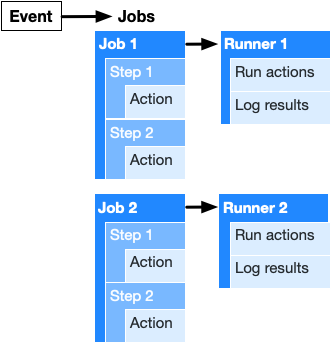
\includegraphics[width = \columnwidth]{./Imagenes/overview-actions-design.png}
    \caption{Diagrama de componentes en GitHub Actions}
\end{figure}

A continuación, se describirán los componentes de GitHub Actions. [2]

\begin{description}
    
    \item[Workflows]
    El flujo de trabajo (\textit{workflow}) es un procedimiento automatizado que agrega a su repositorio. Los flujos de trabajo se componen de uno o más trabajos (\textit{jobs}) y pueden ser programados o activados por un evento (\textit{event}). El flujo de trabajo se puede usar para:
    
    \begin{itemize}
        \item Crear
        \item Probar
        \item Empaquetar
        \item Lanzar
        \item Implementar
    \end{itemize}

    \item[Events]
    Un evento (\textit{event}) es una actividad específica que desencadena un flujo de trabajo. Por ejemplo, la actividad puede originarse en GitHub cuando alguien:

    \begin{itemize}
        \item Ejecuta un \textbf{push}
        \item Crea un problema (\textit{issue})
        \item Crea un \textbf{pull request}
    \end{itemize}

    \item[Jobs]
    Un trabajo (\textit{job}) es un conjunto de pasos (\textit{steps}) que se ejecutan en el mismo \textit{runner}. De forma predeterminada, un flujo de trabajo con varios trabajos ejecutará esos trabajos en paralelo, pero también puede hacerlo de forma secuencial. Por ejemplo, un flujo de trabajo puede tener dos trabajos secuenciales que compilan y prueban código, donde el trabajo de prueba depende del estado del trabajo de compilación. Si el trabajo de compilación falla, el trabajo de prueba no se ejecutará.

    \item[Steps]
    Un paso (\textit{step}) es una tarea individual que puede ejecutar comandos en un trabajo. Un paso puede ser una acción o un comando de shell. Cada paso de un trabajo se ejecuta en el mismo \textit{runner}, lo que permite que las acciones de ese trabajo compartan datos entre sí.

    \item[Actions]
    Las acciones (\textit{actions}) son comandos independientes que se combinan en pasos para crear un trabajo. Las acciones son el bloque de construcción portátil más pequeño de un flujo de trabajo. Es posible crear sus propias acciones o utilizar acciones creadas por la comunidad de GitHub. Para usar una acción en un flujo de trabajo, debe incluirla como un paso.

    \item[Runners]
    Un runner es un servidor que tiene instalada la aplicación de ejecución de acciones de GitHub. Puede utilizar un runner alojado en GitHub, o puede alojar el suyo propio. Un runner escucha los trabajos disponibles, ejecuta un trabajo a la vez e informa el progreso, los registros y los resultados a GitHub. Para los ejecutores alojados en GitHub, cada trabajo de un flujo de trabajo se ejecuta en un entorno virtual nuevo.

    Los runners alojados en GitHub se basan en:

    \begin{itemize}
        \item Ubuntu Linux
        \item Microsoft Windows
        \item macOS
    \end{itemize}


\end{description}

\subsubsection{YAML}

YAML es un lenguaje de serialización de datos diseñado para ser \textit{leído y escrito por humanos}. Basa su funcionalidad en JSON, con la adición de líneas nuevas e indentación inspirada en Python. A diferencia de Python, YAML no permite tabulaciones literales. [3]

Las GitHub Actions utiliza la sintaxis YAML para definir los eventos, trabajos y pasos. Estos archivos YAML se almacenan en el repositorio, en el directorio \textbf{.github/workflows}. [2]

\subsubsection{Ejemplo}

Se puede crear un flujo de trabajo de ejemplo en un repositorio que activa automáticamente una serie de comandos cada vez que se realiza un \textbf{push}. En este flujo de trabajo, GitHub Actions verifica el código enviado, instala las dependencias del software y ejecuta \textbf{bats -v}.

Los pasos para crear este flujo de trabajo son los siguientes:

\begin{enumerate}

    \item Crear un repositorio en GitHub.
    \item Crear un nuevo archivo \textbf{learn-github-actions.yml} en el directorio \textbf{.github/workflows/} con el siguiente código:

\begin{verbatim}
name: learn-github-actions
on: [push]
jobs:
  check-bats-version:
    runs-on: ubuntu-latest
    steps:
      - uses: actions/checkout@v2
      - uses: actions/setup-node@v1
      - run: npm install -g bats
      - run: bats -v
\end{verbatim}

\begin{figure}[h]
    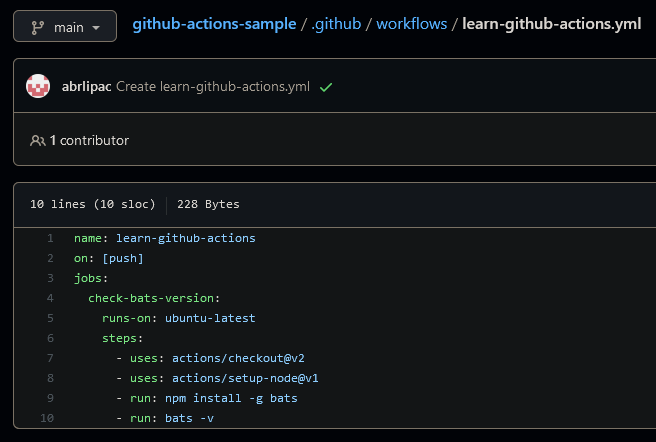
\includegraphics[width = \columnwidth]{Imagenes/Screenshot_1.png}
    \caption{Captura de la ruta del archivo creado}
\end{figure}

    \item Guardar los cambios (\textit{commit})

\end{enumerate}

Cada vez que se haga \textit{push} al repositorio, se ejecutará el flujo de trabajo creado.

Es posible ver la actividad de los flujos en la pestaña \textbf{Actions}. Al abrir un workflow se puede ver los pasos y los logs generados en cada uno.

\begin{figure}[!h]
    \begin{center}
        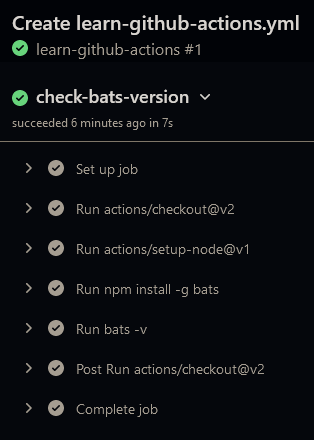
\includegraphics[width = 2in]{./Imagenes/Screenshot_2.png}
        \caption{Captura del flujo de trabajo en la pestaña Actions}
    \end{center}
\end{figure}

\subsubsection{Precios}

El uso de GitHub Actions es gratuito para los repositorios públicos. Para los repositorios privados, cada cuenta de GitHub recibe una cantidad determinada de minutos y almacenamiento gratuitos dependiendo del producto que se utilice con la cuenta.

\begin{table*}[ht]
\begin{center}
\begin{tabular}{|l|l|l|}
\hline
\rowcolor[HTML]{6665CD} 
\multicolumn{1}{|c|}{\cellcolor[HTML]{6665CD}{\color[HTML]{FFFFFF} \textbf{Producto}}} & \multicolumn{1}{c|}{\cellcolor[HTML]{6665CD}{\color[HTML]{FFFFFF} \textbf{Almacenamiento}}} & \multicolumn{1}{c|}{\cellcolor[HTML]{6665CD}{\color[HTML]{FFFFFF} \textbf{Minutos (por mes)}}} \\ \hline
GitHub Free                                                                            & 500 MB                                                                                      & 2,000                                                                                          \\ \hline
GitHub Pro                                                                             & 1 GB                                                                                        & 3,000                                                                                          \\ \hline
GitHub Free para organizaciones                                                        & 500 MB                                                                                      & 2,000                                                                                          \\ \hline
GitHub Team                                                                            & 2 GB                                                                                        & 3,000                                                                                          \\ \hline
GitHub Enterprise Cloud                                                                & 50 GB                                                                                       & 50,000                                                                                         \\ \hline
\end{tabular}
\end{center}
\caption{Tabla de los productos ofrecidos por GitHub, Almacenamiento y minutos mensuales}
\end{table*}

Cada sistema operativo consume una cantidad diferente de minutos, siendo 1 minuto de trabajos ejecutados en Linux equivalente a 1 minuto de facturación mensual.

\begin{table*}[ht]
\begin{center}
\begin{tabular}{|l|l|l|}
\hline
\rowcolor[HTML]{6665CD} 
\multicolumn{1}{|c|}{\cellcolor[HTML]{6665CD}{\color[HTML]{FFFFFF} \textbf{Sistema operativo}}} & \multicolumn{1}{c|}{\cellcolor[HTML]{6665CD}{\color[HTML]{FFFFFF} \textbf{Tasa por minuto}}} & \multicolumn{1}{c|}{\cellcolor[HTML]{6665CD}{\color[HTML]{FFFFFF} \textbf{Multiplicador de minutos}}} \\ \hline
Linux                                                                                           & \$0.008                                                                                      & 1                                                                                                     \\ \hline
macOS                                                                                           & \$0.08                                                                                       & 10                                                                                                    \\ \hline
Windows                                                                                         & \$0.016                                                                                      & 2                                                                                                     \\ \hline
\end{tabular}
\end{center}
\caption{Tabla de los sistemas operativos soportados, la tasa por minuto en dólares y el multiplicador}
\end{table*}

\subsection{Comparación}

\subsubsection{Jenkins y Github Actions}

\textbf{Diferencias}

\begin{itemize}
    \item Jenkins cuenta con pipelines monolíticos y secuenciales como un proceso en cascada, mientras que GitHub Actions cuenta con pipelines asíncronos y basados en componentes como un proceso ágil.
    \item Jenkins no está diseñado para la nube, mientras que GitHub Actions está en la nube (aunque también se puede instalar en un servidor local).
    \item Jenkins requiere una instalación, mientras que GitHub Actions, no.
    \item Jenkins tiene un diseño basado en cuentas y activadores que no se corresponde con un evento de GitHub, mientras que GitHub Actions, en los eventos de GitHub, entre los cuales están: \textit{push, pull, issue, comment, clone, publish}, entre otros.
    \item GitHub Marketplace tiene más de 4,000 acciones lanzadas en menos de dos años. Jenkins ha lanzado más de 1,000 complementos diferentes en aproximadamente diez años.
    \item Jenkins tiene un costo de mantenimiento más alto que GitHub Action.
    \item GitHub Actions es más flexible que Jenkins al ser posible ejecutarlo localmente y enviarlo a GitLab u otro almacenamiento de versiones en la nube.
    \item Jenkins requiere de un servidor dedicado, mientras que GitHub Actions, no.
\end{itemize}

\subsection{Azure DevOps}

\subsubsection{Definicion}

Donovan Brown, el Administrador de DevOps principal en el grupo de Azure lo describe: "DevOps es la unión de personas, procesos y productos para permitir la entrega continua de valor a los usuarios finales".[5]

DevOps permite que los roles que antes estaban aislados (desarrollo, operaciones de TI, ingeniería de la calidad y seguridad) se coordinen y colaboren para producir productos mejores y más confiables.[6]

\subsubsection{Ventajas}

Mejoran el rendimiento y crean productos de más calidad en menos tiempo, lo que aumenta la satisfacción de los clientes. Esta mejora de la colaboración y la productividad es fundamental también para alcanzar objetivos de negocio como estos:

\begin{itemize}
\item Reducción del tiempo de comercialización
\item Adaptación al mercado y a la competencia
\item Mantenimiento de la estabilidad y la confiabilidad del sistema
\item Mejora del tiempo medio de recuperación
\end{itemize}

\subsubsection{DevOps y el ciclo de vida de las aplicaciones}
DevOps influye en el ciclo de vida de las aplicaciones a lo largo de las fases de planeamiento, desarrollo, entrega y uso.

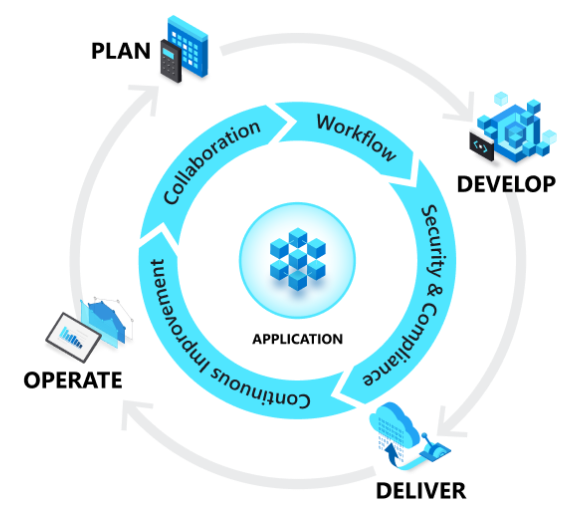
\includegraphics[width = 6cm]{./Imagenes/1.png}


\subsubsection{Herramientas}
- \textbf{GitHub}
Aumenta la colaboración, flujos de trabajo del código\\
- \textbf{Azure Pipelines}
Implementa CI/CD para compilar, probar e implementar soluciones de forma continuada\\
- \textbf{Azure Boards}
Planea, controla el trabajo entre los equipos\\
- \textbf{Azure Monitor}
Visibilidad sobre las aplicaciones, la infraestructura y la red\\
- \textbf{Visual Studio}
IDE diseñado para crear aplicaciones eficaces y escalables para Azure\\
- \textbf{Azure Kubernetes Service}
Distribuye aplicaciones en contenedores con más rapidez

\subsection{Azure Pipeline y GitHub Actions}



\subsubsection{Similitudes}
- Los archivos de configuración del flujo de trabajo se escriben en YAML

- Los flujos de trabajo incluyen uno o más trabajos.

- Los pasos o tareas se pueden reutilizar y compartir con la comunidad.

\textbf{Diferencias entre Azure Pipeline y GitHub Actions}[7]

\begin{figure*}[htb]
\centering
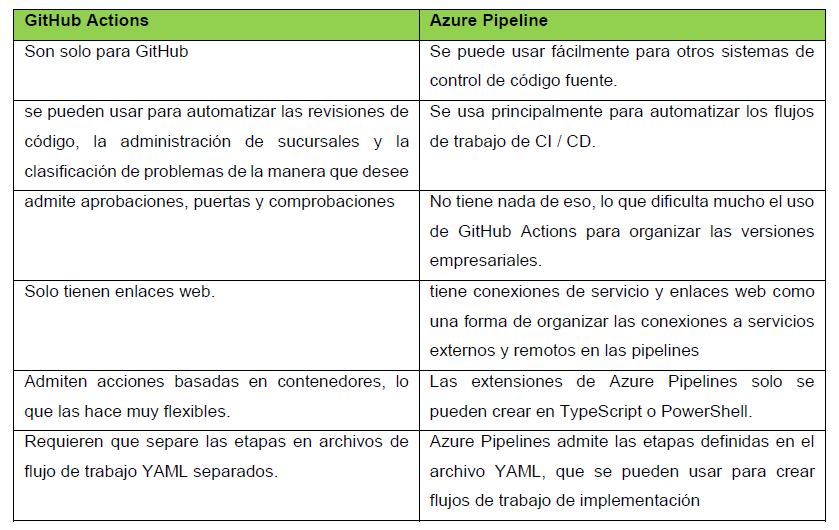
\includegraphics[width=1\textwidth]{./Imagenes/2.png}
\caption{Diferencias entre Azure Pipeline y GitHub Actions}
\label{fig:mont}
\end{figure*}


\begin{figure}[t]
    \begin{center}
        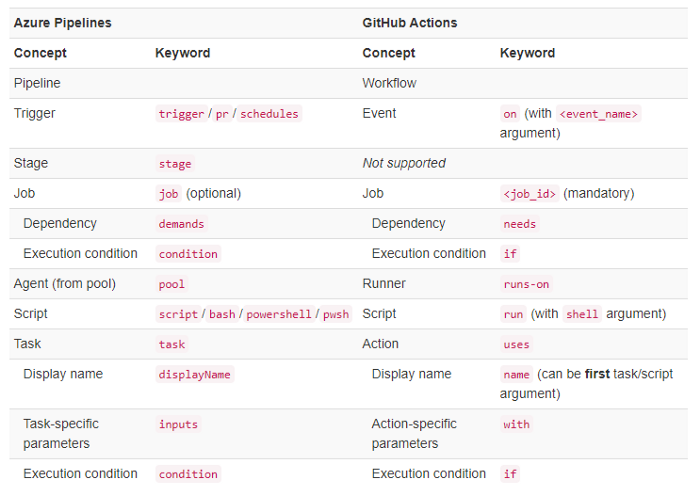
\includegraphics[width = \columnwidth]{./Imagenes/1 iwr4M9D-eSbMV8ki5xbU2w.png}
        \caption{Tabla comparativa de sintaxis de Azure Pipelines y GitHub Actions}
    \end{center}
\end{figure}

%----------------------------------------------------------------------------------------
%	Conclusiones
%----------------------------------------------------------------------------------------

\newpage

\section{Conclusiones}

En conclusión, luego de un análisis, se puede notar que GitHub Actions facilita la creación, prueba e implementación de su código directamente desde GitHub, sin embargo, si se desea utilizar flujos de trabajo de GitHub Action solo para distribución o implementación continua se recomendaría usar Azure Pipelines y sus ya conocidas características para permitir implementaciones seguras y compatibles en los entornos de producción.
Cada proyecto de software realizado y gestionado a través de estas herramientas permitirá una mejor toma de decisiones por parte de la gerencia o dirección de proyectos.
Así mismo, es importante destacar que, para la implementación de la herramienta, se consideran aspectos relevantes en el área de pruebas de software, así como algunas métricas para software, todo esto con el propósito de enriquecer los criterios de evaluación y obtener un producto de calidad.
La realización de este artículo permite entender que la gestión de las pruebas de software es una actividad que indiscutiblemente debe llevarse a cabo en todo proyecto de software.

%----------------------------------------------------------------------------------------
%	Recomendaciones
%----------------------------------------------------------------------------------------

\section{Recomendaciones}


\begin{itemize}
\item Se recomienda verificar todos los cambios antes y después de refactorizar la aplicación. La herramienta elegida debe cumplir con los requisitos para realizar y entregar los resultados esperados.
\item La capacidad de informar errores y fallas es importante para que los desarrolladores puedan reproducir el problema y solucionarlo. Es bueno tomar en cuenta las herramientas que permiten revisar los resúmenes de registro de cada prueba a lo largo de los plazos.
\item La herramienta elegida siempre debe probar nuevos cambios de código y brindar retroalimentación. Una herramienta de prueba sólida debe tener la capacidad de admitir el marco de prueba, el control de revisión, la gestión de configuración de prueba, el seguimiento de problemas, la generación de informes y más.


\end{itemize}



%----------------------------------------------------------------------------------------
%	BIBLIOGRAFIA
%----------------------------------------------------------------------------------------

\selectlanguage{spanish}
\begin{thebibliography}{99} 

\bibitem[1]{}
\newblock GitHub. (s. f.). Documentación de GitHub Actions - GitHub Docs. GitHub Actions. Recuperado 9 de enero de 2021, de https://docs.github.com/es/free-pro-team@latest/actions
\bibitem[2]{}
\newblock GitHub. (s. f.-b). Introduction to GitHub Actions - GitHub Docs. Introduction to GitHub Actions. Recuperado 9 de enero de 2021, de https://docs.github.com/es/free-pro-team@latest/actions/learn-github-actions/introduction-to-github-actions
\bibitem[3]{}
\newblock Leigh Brenecki, L. B. (s. f.). Learn yaml in Y Minutes. Aprende X en Y minutos Donde X=yaml. Recuperado 9 de enero de 2021, de https://learnxinyminutes.com/docs/es-es/yaml-es/
\bibitem[4]{}
\newblock GitHub. (s. f.-a). Acerca de la facturación para GitHub Actions - GitHub Docs. Acerca de la facturación para GitHub Actions. Recuperado 9 de enero de 2021, de https://docs.github.com/es/free-pro-team@latest/github/setting-up-and-managing-billing-and-payments-on-github/about-billing-for-github-actions
\bibitem[5]{}
\newblock Cottman, B. H. (2020, 9 julio). Will Github Actions Kill off Jenkins? - The Startup. Medium. https://medium.com/swlh/will-github-actions-kill-off-jenkins-f85e614bb8d3
\bibitem[6]{}
\newblock Yermakhanov, M. (2020, 11 diciembre). Azure Pipelines vs. GitHub Actions: Key Differences. Medium. https://medium.com/objectsharp/azure-pipelines-vs-github-actions-key-differences-45390ab132ee

\end{thebibliography}


%----------------------------------------------------------------------------------------


\end{document}
